\section{Runtime cost comparison on a real-world MeerKAT reconstruction}\label{scale}
Current Compressed Sensing reconstructions produce images at a higher quality than CLEAN. However, CLEAN is significantly cheaper to compute. MeerKAT's large scale reconstruction problems, CLEAN is still the go-to algorithm. In this project, we developed for a new architecture, which uses the relevant columns of the Fourier Transform Matrix directly. We developed a Coordinate Descent algorithm with this architecture and demonstrated in section \ref{results} super-resolution performance on simulated data. The question, if we can lower the runtime costs with our new architecture, is still open. 

In this section, we compare the costs of Coordinate Descent with WSCLEAN, which is the reconstruction algorithm of choice for MeerKAT reconstructions. We create cost functions for each algorithm, which estimate the number of operations depending on the input size. WSCLEAN was executed on a real-world MeerKAT dataset shown in image \ref{scale:wsclean}. Our proof-of-concept implementation was not able to handle the large amount of data. Instead, we extrapolate the best-case costs of our approach and compare them to WSCLEAN on the MeerKAT dataset.


\subsection{Cost function of an idealized Coordinate Descent}
The runtime cost of Coordinate Descent depends on the number of Visibilities $M$ and the number of non-zero starlets $S$. The number and location of the $S$ non-zero starlets are generally not known. However, we created a heuristic which finds likely non-zero starlet components. In a realistic setting, the heuristic will have found more than $S$ likely non-zero starlets. For the idealized version of Coordinate Descent, we assume an oracle performance heuristic: It finds the location and number of the $S$ non-zero starlet components in constant time. Coordinate Descent therefore has to calculate the value of $S$  components. In total, the idealized Coordinate Descent algorithm uses four steps: creating $J$ starlet levels with the non-uniform FFT, creating the columns of $F^{-1}$, calculating the minima for each single component, and calculating the starlet layers:

\begin{alignat*}{1}
J \text{non-uniform FFTs for the starlet regularization} &: J*(M + 2N*ld(2N))\\
\text{creating} \:S\: \text{columns of}\: F^{-1} &: S*7M\\
\text{locating} \:S\: \text{minima of} \:S\: \text{parabolas} &: S*4M\\
\text{calculating} \:J\: \text{Starlet layers} &: J * 2M
\end{alignat*}

We assume we have enough memory to cache the columns of $F^{-1}$ and only need to calculate them once. Keep in mind that each column of $F^{1}$ has the same length as the Visibilities, essentially multiplying the input data. The last parameter for Coordinate Descent is the number of iterations to converge, $I_CD$. Estimating this number is difficult as Coordinate Descent does not have strict guarantees (as discussed in section \ref{cd}). Instead, we assume it converges after a fixed number of iterations. Therefore we arrive at the cost function of \eqref{results:cd:omega}.

\begin{equation}\label{results:cd:omega}
\begin{aligned}
	CD(I_{CD}, M, S, J) = &I_{CD} * [S * 4M + J * 2M]\\
		&+  S*7M\\
		&+ J*(M + 2N*ld(2N))
\end{aligned}
\end{equation}

Note that the runtime of Coordinate Descent is independent of the number of pixels. The only image related parameter in \eqref{results:cd:omega} is $J$, the number of starlet layers. The largest starlet layer represents the largest possible structure in the image, which is given by the instrument and the image resolution. The runtime only depends indirectly on the image resolution, not the total number of pixels. For simplicity, we assume the image cannot have structures larger than half the image size. For our MeerKAT example, this is more than enough to represent the largest structures.

Also note the term iterating over the $S$ non-zero starlets, $ I_{CD} * [S * 4M +\ldots]$. As it turns out, this is the Achilles heel of the algorithm. MeerKAT observations contain a very large amount of Visibilities $M$.

\subsection{Cost function of WSCLEAN}
The WSCLEAN algorithm uses the Major Cycle architecture. It uses the non-uniform FFT with $w$-stacking. The runtime costs of a single Major Cycle depends on the non-uniform FFT with $w$-stacking and the number of CLEAN deconvolutions. $N$ denotes the number of pixels.

\begin{alignat*}{1}
	\text{non-uniform FFT} &: M + 2N*ld(2N)\\
	\text{non-uniform FFT with} \:w\text{-stacking} &:M + W*(2N*ld(2N) + 2N) + N*ld(N)\\
	I_{CLEAN}\: \text{deconvolutions} &: I_{WSCLEAN}*2N
\end{alignat*}

The overall cost function shown in \eqref{results:clean:o} can also be split into two parts. In each Major Cycle, the forward and backwards non-uniform FFTs gets calculated, and CLEAN deconvolves the image for a maximum number of $I_{CLEAN}$ deconvolutions.

\begin{equation}\label{results:clean:o}
\begin{aligned}
 WSCLEAN(I_{Major}, I_{CLEAN}, M, N,  W) =\: &I_{Major} * 2 * [M + W*(2N*ld(2N) + 2N) + N log N]\\
	&+ [I_{CLEAN}*2N]
\end{aligned}
\end{equation}

Notice that the number of CLEAN deconvolutions $I_{CLEAN}$ depends on the image content, similar the number of non-zero starlets $S$ for Coordinate Descent. Here however, it multiplies with the number of pixels instead of the number of Visibilities. In a sense, the major cycle tries to reduce the runtime complexity of handling the image content by calculating the non-uniform FFT. If the difference is large enough $N \ll M$, then the Major Cycle will end up with a smaller runtime costs.


\subsection{Comparison on a MeerKAT reconstruction problem}
Our real-world MeerKAT observation has been calibrated and averaged in frequency and time to reduce storage space. The resulting dataset contains 540 channels with 4 million Visibilities each. Due to hardware limitations, WSCLEAN was calculated on 75 channels. The reconstructed image is shown in \ref{scale:wsclean}, and the resulting parameters for our cost function are: 
\begin{itemize}
	\item Major Cycles: $I_{Major} = 6$
	\item Number of CLEAN iterations: $I_{CLEAN} = 35'000$
	\item Visibilities: $M=3.05e^8$
		\item Pixels: $N = 2048^2$
	\item $w$-stacks: $W = 32$
\end{itemize}

\begin{figure}[h]
	\centering
	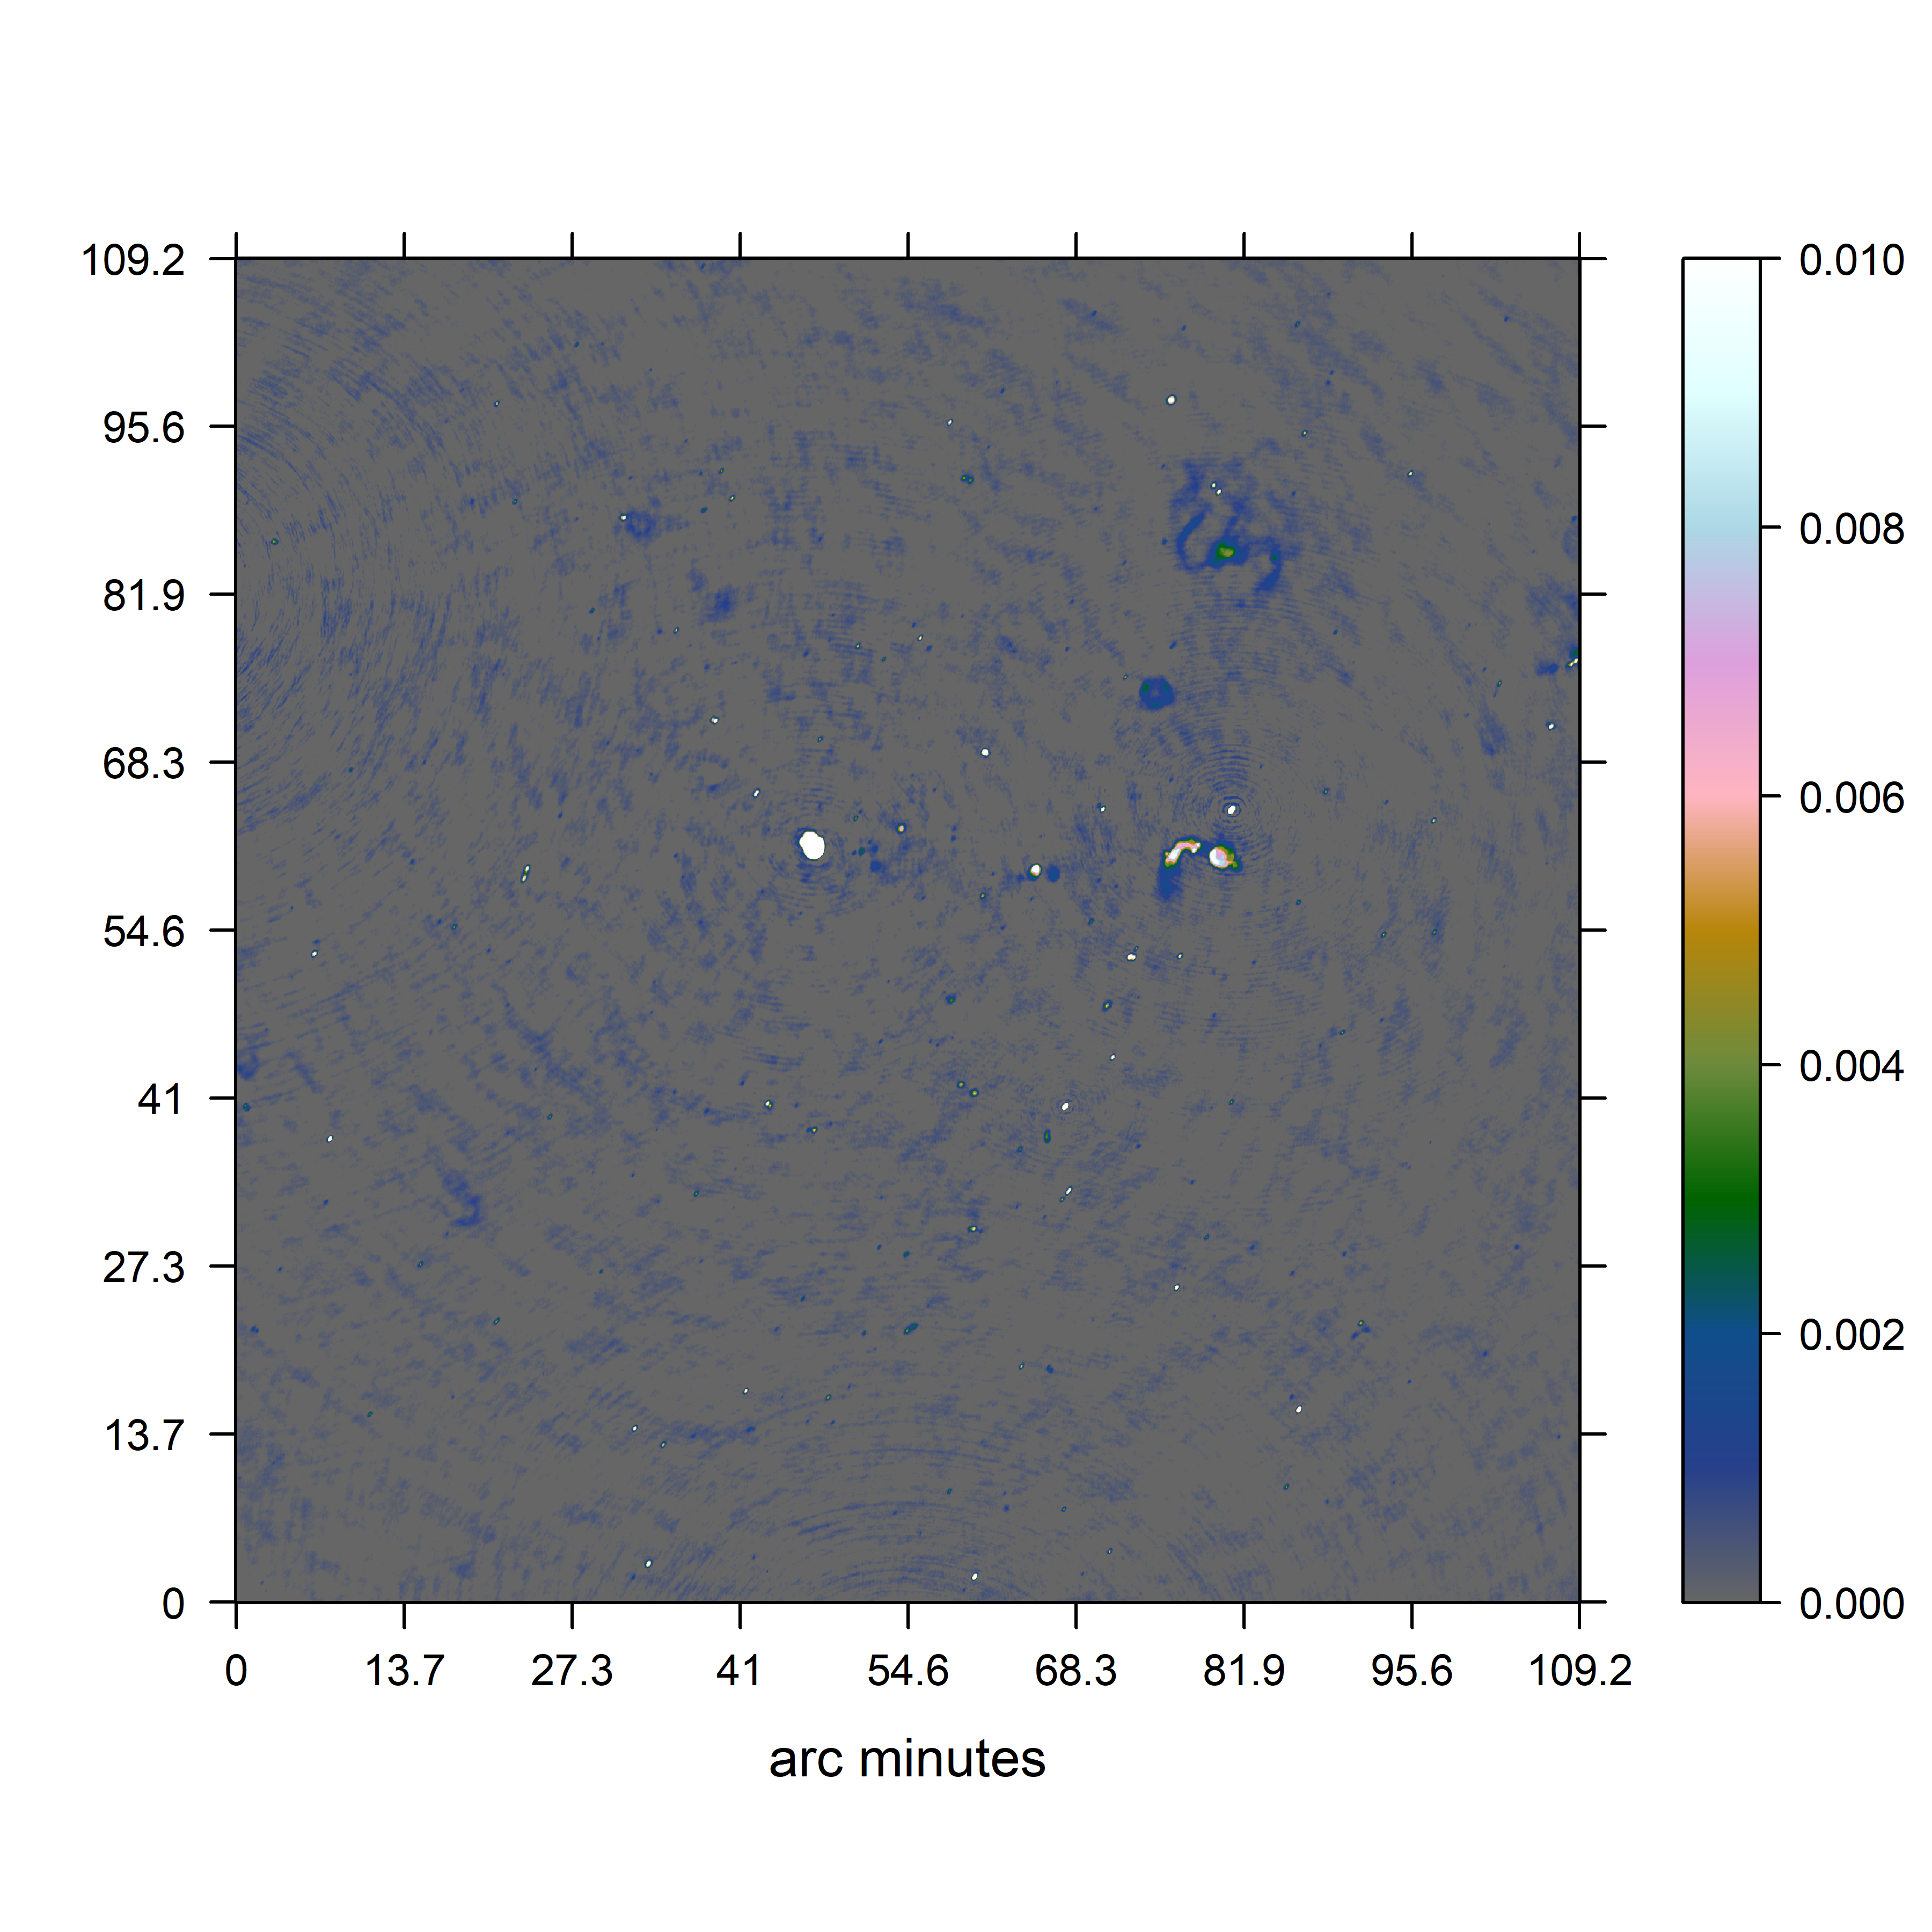
\includegraphics[width=0.6\linewidth]{./chapters/21.scalability/meerkat.png}
	\caption{WSCLEAN Reconstruction of the MeerKAT observation.}
	\label{scale:wsclean}
\end{figure}

For Coordinate Descent's costs, we need an estimate for $J$, $S$ and $I_{CD}$. We set $J=8$, which lets the largest structure span over half the image, enough to capture any large scale structures. For $S$ and $I_{CD}$, we simply use the values from our simulated reconstruction \ref{results:mixed:cd} and set $S=250$ and 
$I_{CD}=10$. This is an under-estimation of the true values. The image \ref{scale:wsclean} shows complex-shaped extended emissions, which likely needs a larger number of starlets for representation than the Gaussian emissions from our simulation. 

When we put all values into our cost functions \eqref{results:cd:omega} and \eqref{results:clean:o}, Coordinate Descent with the direct Fourier transform arrives at 9.7 times the costs of WSCLEAN in the best case scenario. Our approach has not reduced the runtime costs compared to WSCLEAN. But what about Major Cycle Compressed Sensing algorithms? We have not developed a cost function for other Major Cycle approaches, but we can get a very rough estimate by changing $I_{Major}$ of the WSCLEAN cost function. Pratley et al.\cite{pratley2018fast} reported 10 Major Cycles for a Compressed Sensing reconstruction on simulated data. If we plug in 10 Major Cycles for WSCLEAN, Coordinate Descent ends up taking roughly 8 times the cost of the Major Cycle algorithm. Mind you these costs are only valid when we can keep all necessary columns of $F$ in memory, eating up 1.1 terabytes\footnote{If we assume 64 bit floating point accuracy for the real and complex values of the Visibilities.} in our case. If not, the columns have to be re-calculated on the fly, increasing the runtime costs by magnitudes. 

The issue with Coordinate Descent's runtime complexity lies in the term $I_{CD} * [S * 4M +\ldots]$ of \eqref{results:cd:omega}, which scales with the "content" of the image $S$, multiplied with the Visibilities. Coordinate Descent cannot afford many iterations nor many non-zero components, because both of these numbers get multiplied together with $M$, the largest number in the problem. With the Major Cycle architecture, WSCLEAN is able to get around this limitation, and scales any content dependent factors on $N$ instead of $M$. 

Indeed, the runtime of our Coordinate Descent algorithm could be improved by using the Major Cycle architecture, essentially replacing $M$ with $N$ and we arrive at the term $I_{CD} * [S * 4N +\ldots]$. In this case Coordinate Descent can afford more iterations and more non-zero components for the same runtime costs. Furthermore $N$ lies on a uniformly sampled grid. We may be able to use the FFT instead of caching columns of $F$, and reduce the memory requirement at the same time.


\subsection{Approximations as key for going large scale}
We set out to reduce the runtime costs of compressed Sensing reconstructions by replacing the non-uniform FFT approximation. Ironically we ended up with an algorithm which not only has higher runtime costs, the costs may even be reduced by moving back to the Major Cycle architecture. 

The question arises, whether the direct Fourier Transform has a future for MeerKAT reconstructions or not. From the current results we can summarize that the Major Cycle architecture with the non-uniform FFT is a good approximation of the Fourier Transform with no clear alternative. The emphasis is on the approximation. We do not need an exact transform. The Visibilities are inherently noisy, and even with the optimal reconstruction there will be residual noise in the image above the level of floating point accuracies. An optimal Fourier Transform for MeerKAT takes the inherent inaccuracy into account.

The direct Fourier Transform, as it is implemented in our algorithm, wastes resources with a precise transformation. In the context of MeerKAT, it has to re-introduce approximations to be competitive. Our Coordinate Descent approach leveraged the fact that not all columns of $F$ are necessary for reconstruction. The next step is to see if the number of rows can be reduced too.

A MeerKAT reconstruction has magnitudes fewer pixels than Visibilities. Not all samples contribute the same amount of information to a reconstruction.If we can remove the redundant information before reconstruction, we can reduce the overall costs and increase the ratio of samples per pixel. Our Coordinate Descent algorithm scales independently of image size, the fewer samples we have per pixel, the more cost effective our algorithm becomes compared to CLEAN.

As it is, our proof-of-concept algorithm with the direct Fourier Transform is too expensive when compared to CLEAN. It wastes resources on a too precise transformation. By re-introducing approximations, we can further decrease the runtime costs of the direct Fourier Transform. Whether we can find an approximation, which is at least as accurate as the non-uniform FFT and has lower runtime costs remains to be investigated in the future.


















 